\chapter{Functional Decomposition and Solutions}
% this is some introduction about the topic
\subsection{Pre-class Activities}
\subsubsection{Activity 1: Decompose the Problem}
\textbf{Objective:} \\

The objective of this activity is to analyse the selected product's primary functions and decomposing the problem to identify its major components or subsystems. By documenting the chosen approach for problem decomposition and creating function diagrams, you will gain a clearer understanding of the product's functional elements and their relationships.

\begin{enumerate}
    \item Analyze the product's primary functions and identify the major components or subsystems that contribute to its operation.
    \begin{enumerate}
        \item This step involves gaining a clear understanding of the overall function of the product.
    \end{enumerate}
    \item Choose one of the following approaches for problem decomposition:
    \begin{enumerate}
        \item Functional Decomposition
        \item Decomposition by Sequence of User Actions
        \item Decomposition by Key Customer Needs
    \end{enumerate}
    \item Document (justify the selection) the chosen approach for problem decomposition and apply it to the selected product.
    \begin{enumerate}
        \item Use appropriate diagrams, such as function diagrams or flowcharts, to visually represent the decomposition process and the relationships between different components or subfunctions.
        \item Make sure to use VERB when expressing the functional element of the individual operation and operation.
        For example
        \begin{itemize}
            \item Make Coffee
            \item Extract Coffer
            \item Keep Coffee
            \item Warm Water
            \item Move Water
            \item Give Heat
        \end{itemize}
    \end{enumerate}
    \item Also, it is wise to have a write up about how the functional element works for ease of understanding
    \item Note that at this stage the goal is to describe the functional elements of the product without implying a specific technological working principle for the product concept.
    \item Save the output as a PDF when submitting to ITEL
\end{enumerate}

\subsubsection{Activity 2: Search and Find Solutions} % if available
\textbf{Objective:} \\ 
The objective of this activity is to walk you in executing comprehensive searches and gathering solutions for critical sub-problems related to the selected product and ultimately the finding may help you in generating concepts that ensure the product's smooth functionality.

\textbf{Procedure:}
\begin{enumerate}
    \item To conduct an external search, you may consider sources such as academic publications, industry reports, technical journals, and relevant online platforms.
    \begin{enumerate}
        \item The combination between search engine and appropriate search keywords/phrases that are specific to each sub-problem may help in pinpointing/retrieving relevant information.
    \end{enumerate}
    \item Jot down and compile at least five different solutions for each critical sub-problem obtained from the external/internal search.
    \begin{enumerate}
        \item For the benefit of other reader (your team member, and module convener), it is strongly recommended to details, such as the source, author, publication date, and a brief description of each solution.
    \end{enumerate}
\end{enumerate}

\subsection{In-class Activities}
\subsubsection{Activity 1: Decompose the Problem}
Compile all findings and discuss with all members to determine the best approach to decompose the problem into its major components or subsystems. Each member should explain their selection to their team members. Once consensus is reached, choose one of the following approaches for problem decomposition:
\begin{enumerate}
    \item Functional Decomposition
    \item Decomposition by Sequence of User Actions
    \item Decomposition by Key Customer Needs
\end{enumerate}


\begin{figure}[h!]
\centering
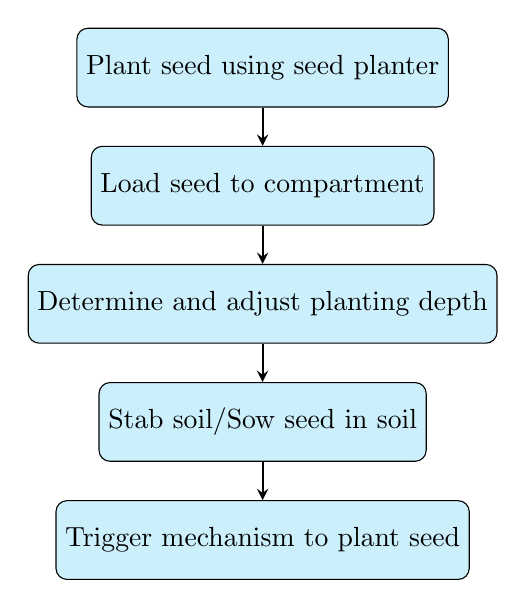
\begin{tikzpicture}[node distance=1.5cm]

\tikzstyle{startstop} = [rectangle, rounded corners, minimum width=3cm, minimum height=1cm,text centered, draw=black, fill=cyan!20]
\tikzstyle{arrow} = [thick,->,>=stealth]

\node (start) [startstop] {Plant seed using seed planter};
\node (load) [startstop, below of=start] {Load seed to compartment};
\node (depth) [startstop, below of=load] {Determine and adjust planting depth};
\node (stab) [startstop, below of=depth] {Stab soil/Sow seed in soil};
\node (trigger) [startstop, below of=stab] {Trigger mechanism to plant seed};

\draw [arrow] (start) -- (load);
\draw [arrow] (load) -- (depth);
\draw [arrow] (depth) -- (stab);
\draw [arrow] (stab) -- (trigger);

\end{tikzpicture}
\caption{Minimum planting layout in Session 8}
\label{fig:planting_flowchart}
\end{figure}


or another example of functional decomposition



\begin{minted}[
  fontsize=\small,
  linenos,
  breaklines=true,
  frame=lines,
  label=code:importJson
]{text}
Manual Seed Planter System
├── Efficient Seed Storage and Dispensing Mechanism
│   ├── Seed Metering Plate
│   ├── Seed Metering Drum
│   ├── Auger-Based Funnel
│   ├── Vibratory Feeder
│   ├── Gravity Feed Chute
│   ├── Belt Conveyor with Seed Pockets (belt with holes carrying seeds)
│   ├── Air Suction Pickup (vacuum picks and releases single seeds)
│   ├── Peristaltic Tube Dispenser (seeds squeezed along flexible tubing)
│   └── Cartridge Loading System (pre-loaded seed cartridges)
│
├── Efficient Seed Sowing
│   ├── Syringe Tip Dispensing
│   ├── Spring Loaded Gate
│   ├── Flap Valve Mechanism
│   ├── Rotating Nozzle Dispenser
│   ├── Telescopic Tube Dispenser (tube that extends downward to sow)
│   ├── Flexible Nozzle Guide (rubbery nozzle that can be aimed precisely)
│   ├── Motorized Dropper (electric controlled seed dropping)
│   └── Gravity Dropper Tube (simple tube relying on gravity but with guidance)
│
└── Planting Depth Control
    ├── Adjustable Depth Control Plate
    ├── Depth Sensor Gauge
    ├── Wheel-Based Depth Setter
    ├── Adjustable Skid Shoe
    ├── Spring-Loaded Plunger (presses the seed to a set depth)
    ├── Soil Contact Sensor (detects soil pressure to adjust depth automatically)
    ├── Telescopic Arm Adjustment (manual or motorized telescoping arm)
    └── Mechanical Stopper Rod (preset rod that limits downward travel)
\end{minted}


\subsubsection{Activity 2: Generate requirement vs function matrix.
}



Once a comprehensive list of project functions has been identified, the next crucial step is to assess how well these functions align with customer needs. It is equally important to ensure that the number of functions is balanced — sufficient to cover all requirements without introducing unnecessary complexity.

To systematically perform this evaluation, we develop a Requirement vs Function Matrix as shown in Table \ref{tab:req_matrix_table}. This matrix provides a clear and organized method for mapping each customer requirement to the corresponding functions intended to fulfill them. It serves as a visual "roadmap," illustrating the connection between what needs to be achieved and how it will be accomplished.







\input{session9/rfm_table_landscape}

\subsubsection{Activity 3: Search and Find Solutions} % if available
Compile all findings and discuss with all members to determine whether it is more advantageous to select the best different solutions for each critical sub-problem obtained from the external/internal search drafted by one of the members, or to combine findings from all team members. Once consensus is reached, compile at least five different solutions for each critical sub-problem obtained from the external/internal search that reflect the collective agreement of all team members.


